%%%%%%%%%%%%%%%%%%%%%%%%%%%%%%%%%%%%%%%%%
% University Assignment Title Page 
% LaTeX Template
% Version 1.0 (27/12/12)
%
% This template has been downloaded from:
% http://www.LaTeXTemplates.com
%
% Original author:
% WikiBooks (http://en.wikibooks.org/wiki/LaTeX/Title_Creation)
%
% License:
% CC BY-NC-SA 3.0 (http://creativecommons.org/licenses/by-nc-sa/3.0/)
%
%%%%%%%%%%%%%%%%%%%%%%%%%%%%%%%%%%%%%%%%%
%\title{Title page with logo}
%----------------------------------------------------------------------------------------
%	PACKAGES AND OTHER DOCUMENT CONFIGURATIONS
%----------------------------------------------------------------------------------------

\documentclass[12pt]{article}
\usepackage[english]{babel}
\usepackage[utf8x]{inputenc}
\usepackage{natbib}
\usepackage{amsmath}
\usepackage[colorinlistoftodos]{todonotes}
\usepackage{listings}
\usepackage{color}
\usepackage[explicit]{titlesec}
\usepackage{url}
\usepackage{subfig}
\usepackage{graphicx}
\usepackage{grffile}
\usepackage{mwe}

\titleformat{\section}{\normalfont\Large\bfseries}{Experiment \thesection}{1em}{}

\definecolor{dkgreen}{rgb}{0,0.6,0}
\definecolor{gray}{rgb}{0.5,0.5,0.5}
\definecolor{mauve}{rgb}{0.58,0,0.82}

\begin{document}

\begin{titlepage}

\newcommand{\HRule}{\rule{\linewidth}{0.5mm}} % Defines a new command for the horizontal lines, change thickness here

\center % Center everything on the page
 
%----------------------------------------------------------------------------------------
%	HEADING SECTIONS
%----------------------------------------------------------------------------------------

\textsc{\LARGE University of St Andrews}\\[1.5cm] % Name of your university/college
\textsc{\Large CS4103 Coursework 1}\\[0.5cm] % Major heading such as course name
\textsc{\large }\\[0.5cm] % Minor heading such as course title

%----------------------------------------------------------------------------------------
%	TITLE SECTION
%----------------------------------------------------------------------------------------

\HRule \\[0.4cm]
{ \huge \bfseries Middleware}\\[0.4cm] % Title of your document
\HRule \\[1.5cm]
 
%----------------------------------------------------------------------------------------
%	AUTHOR SECTION
%----------------------------------------------------------------------------------------


\Large \emph{Author:}\\
 \textsc{150008022}\\[3cm] % Your name

%----------------------------------------------------------------------------------------
%	DATE SECTION
%----------------------------------------------------------------------------------------

{\large \today}\\[2cm] % Date, change the \today to a set date if you want to be precise

%----------------------------------------------------------------------------------------
%	LOGO SECTION
%---------------------------------------------------------------------------------------


\includegraphics[width = 3.1cm]{images/standrewslogo.png}
 
%----------------------------------------------------------------------------------------

\vfill % Fill the rest of the page with whitespace

\end{titlepage}

\part*{Goal}

The goal of this practical was to implement a distributed application using communication middleware to collect data on user responses to the n-person prisoner's dilemma.

\part{Communication Set-Up}

The application was set up using Spring Initializr \cite{springinit}, which provided a Spring Boot application template, with the web and test starter dependencies. A controller class to provide REST request mappings was implemented, and the test connection method was created in the ProsecutorService class. Unit tests were written for both, and Postman was used to test the request when the application server was running, and to fulfill the criteria for part one.

To provide a user-friendly client, create-react-app \cite{createreactapp} was used to boostrap a react.js application. By using a proxy setting, CORS issues were avoided while developing locally. A simple test button was supplied that would perform an asynchronous call to the API test endpoint, and then print the response to the screen (Figures \ref{fig:beforepress} and \ref{fig:afterpress}). When building distributed systems, it is advised to always design for failure, and so a clear "Failed to Connect" message is shown to the user if the request fails for whatever reason.

\begin{figure}[!ht]
    \centering
    \begin{minipage}{0.45\textwidth}
        \centering
        
\includegraphics[width=0.9\textwidth]{images/part1pretest} % first figure itself
        \caption{Before Press}
        \label{fig:beforepress}
    \end{minipage}\hfill
    \begin{minipage}{0.45\textwidth}
        \centering
        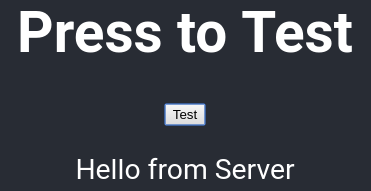
\includegraphics[width=0.9\textwidth]{images/part1posttest} % second figure itself
        \caption{After Press}
        \label{fig:afterpress}
    \end{minipage}
\end{figure}

\part{Single Client Game}

First, the Persecutor service in the Spring Boot application was extended to include the \emph{chooseOption} method, which would take the choice of prisoner one and return the number of years reduction based on a random choice from prisoner two. To reliably test all outcomes produced the desired result when using a random choice generator, the random choice was provided through a separate service which could then be mocked in tests. 

Since only one game would exist at this stage, the endpoint \url{/prosecutor/games/1/prisoners/1} was chosen to be where the prisoner would send their choice in the JSON format. By PUTing their choice to this endpoint, the user could expect a return value of the number of years reduction. 
 		
Spring boot provided the (de)serialization between JSON and the Java object representation through the Jackson library. 

\part{Multiple Client Game - Server}

As an extension, the system was made to handle multiple games. This was first done by extending the persecutor service API.

Given REST design relies on URLs mapping directly to resources, the first step was to design the URL structure in a way that would work for multiple games with multiple prisoners. A hierarchial structure was chosen, where games could be accessed by their ID, prisoners could be accessed by their ID and the game ID they belong to, and so on. Consistency in behaviour was essential, and so a HTTP GET to \url{/prosecutor/games} would return all games and all their prisoners, then \url{/prosecutor/games/1} would return game 1 and all its prisoners, \url{/prosecutor/games/1/prisoners} would only return the list of prisoners from game 1, and \url{/prosecutors/games/1/prisoners/1} would only return prisoner 1 from game 1. The full set of URLs can be found at \url{/swagger-ui.html} when the application is running, along with documentation which describes the JSON output structure and all the supported operations for each URL (Figure \ref{fig:swagger}). 

\begin{figure}[!ht]
        \centering
        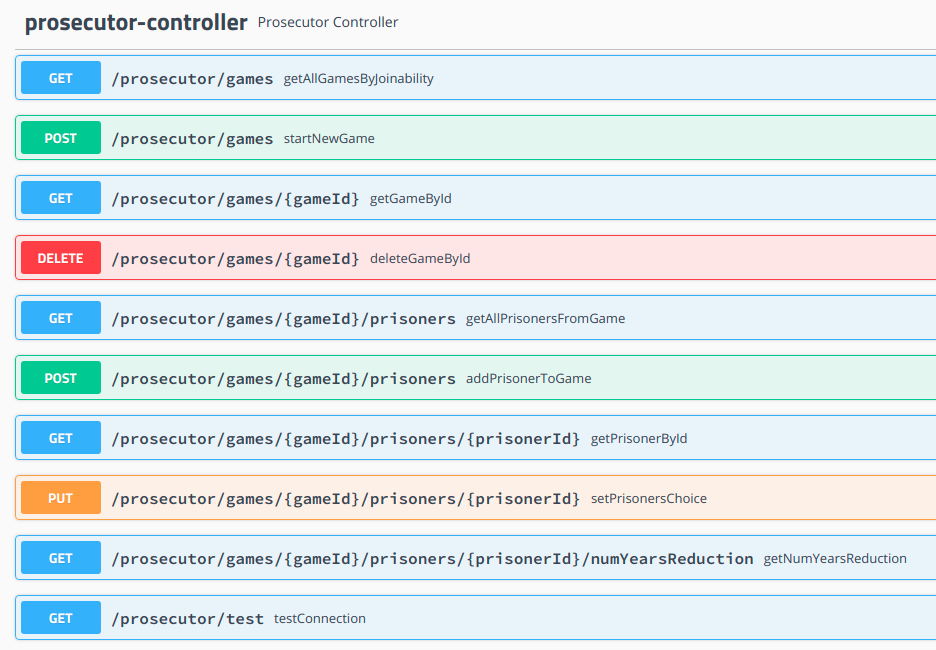
\includegraphics[width=0.8\textwidth]{images/swagger}
        \caption{Swagger Documentation}
        \label{fig:swagger}
\end{figure}

In order to make the API friendlier to use, error messages were standardised such that any exception thrown by the service would provide a HTTP status code and a message for the user, which would then be sent in the response as JSON. This behaviour was tested for using \emph{mockMvc} in \emph{ProsecutorConrollerTest}. Validation was used for any method that took client input.

Though a production ready implementation would use a seperate database server, for this practical a simple H2 in-memory database was used. The repository abstraction provided by Spring Data would mean that with some simple configuration, an external database could be used instead. 

The ProsecutorService was extended to provide all the functonality needed for each controller method, such as getting all games, getting a prisoner from a game, creating a new game, and so on. Unit tests were written for each method by mocking the repositories used. For the repository layer, only the custom queries were tested, as the framework supplied the rest (\url{save, findById, findAll}). 

In order for the client to join a random game, an optional URL parameter was added to the GET request for all games that would allow the client to filter for 'joinable' games. Joinability in this context is any game that can accept at least another prisoner.

The games kept the same structure, where there would be two prisoners per game. Since REST prohibits the use of any kind of session, the client would have to use a polling mechanism to get their years reduction once providing their choice. Message based middleware avoids this issue. For example, a commonly used publish-subscribe messaging protocol middleware provided by Spring Websockets, called STOMP, would allow the client to subscribe to their prisoners status, and allow the server to push the number of years reduction to the client once they became available. REST on the other hand avoids all the overhead involved in maintaining subscriptions and message brokers. The structure of REST APIs also tends to encourage decoupling from any client application, which is useful if the service is ever to be expanded or used differently.

Since the prisoner ID is unique for all prisoners across all games, it would be possible to establish a many-to-many relationship between games and prisoners. Since the heirarchial structure was easier to capture in a REST url design, this functionality was not provided. If it was to be used, a HATEOAS architecture would likely be preferred, where \url{/prisoners} would return a prisoner object with the URLs of all games they partake in, and \url{/games} would return a game object with the URLs of all the prisoners taking part in them. This would avoid cycles in the JSON response objects, and provides what is sometimes referred to as the "final level" of REST.

Given more time, integration tests that would test normal and malicious use patterns would also have been implemented. 

\part{Multiple Client Game - Client}

With the backend API tested and running, the client would now be able to start and join games. Since games used unique identifiers, players could start a game and share their game ID, to allow other players to join. This could be useful in an expiriment, as it could be used to track which participants took part in which games if they are supplied their game and prisoner IDs beforehand. 

The game menu (Figure \ref{fig:startmenu}) provides three options: test connection, join game, and start game. Test connection allows the client to check that the REST server is available before continuing, and to fulfill part one of the practical specification. 

\begin{figure}[!ht]
        \centering
        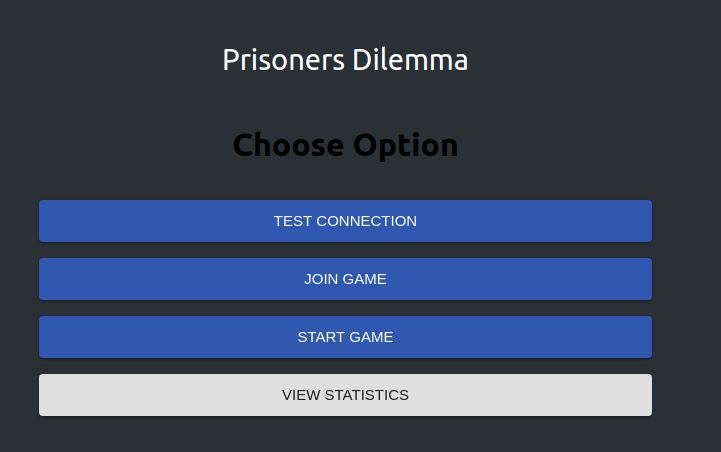
\includegraphics[width=0.5\textwidth]{images/menu} % first figure itself
        \caption{Start Menu}
        \label{fig:startmenu}
\end{figure}

Join game allows the user to either join a random game, or join a specific game by providing a game id and/or a specific prisoner id. The random game feature uses the 'joinable' filter from earlier, and shows an appropriate error message if there are no joinable games. 

\begin{figure}[!ht]
        \centering
        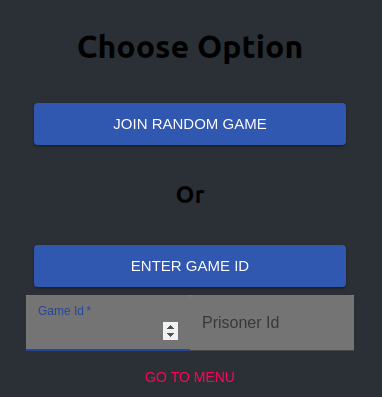
\includegraphics[width=0.5\textwidth]{images/joingame} % first figure itself
        \caption{Join Game Menu}
        \label{fig:joingame}
\end{figure}

If able to join a game, the user is then taken to the choice buttons screen (Figure \ref{fig:makechoice}) where they can see their prisoner and game id.

\begin{figure}[!ht]
        \centering
        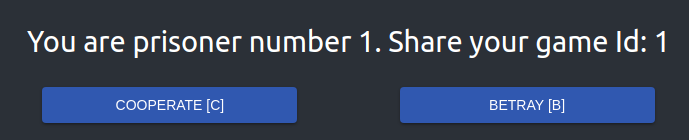
\includegraphics[width=0.5\textwidth]{images/makechoice} % first figure itself
        \caption{Choice Buttons}
        \label{fig:makechoice}
\end{figure}

Start game allows the user to begin a new game, and immediately moves to the choice buttons screen. Once the player has made their decision, the client will begin polling the server for the number of years reduction (Figure \ref{fig:polling}). 

In order to prepare for possible failure, prisoners who started a game and disconnected for whatever reason can return to the game to make their choice at a later time by rejoining with their game and prisoner Id. The same can be done if they experience a failure while waiting for the other prisoner, and in this case they will either be immediately shown the result of their choice, or the polling message screen.

\begin{figure}[!ht]
        \centering
        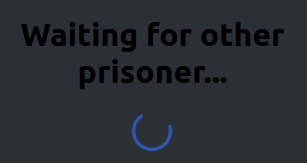
\includegraphics[width=0.5\textwidth]{images/polling} % first figure itself
        \caption{Polling Screen}
        \label{fig:polling}
\end{figure}

To try and minimise server load, the polling mechanism uses random exponential back off with a cap to avoid ridiculous waiting times. The wait time begins at 2 seconds, and is multiplied by a random number between 1 and 2 after every failed try, and reset to 2 seconds after the time reacahes 7 seconds. This jitter is included to avoid stampedes when all clients experience failure at the same time and their polling times become synchronized, which could be catastraphic for the server. A graph of the network activity while polling is shown in Figure \ref{fig:jitter} which demonstrates the jitter with backoff.

\begin{figure}[!ht]
        \centering
        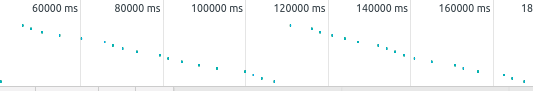
\includegraphics[width=\textwidth]{images/jitter} % first figure itself
        \caption{Exponential back-off with jitter}
        \label{fig:jitter}
\end{figure}

\part*{Conclusion}

\bibliographystyle{unsrt}
\bibliography{mybib}

\end{document}
